% Options for packages loaded elsewhere
\PassOptionsToPackage{unicode}{hyperref}
\PassOptionsToPackage{hyphens}{url}
%
\documentclass[
]{article}
\usepackage{amsmath,amssymb}
\usepackage{lmodern}
\usepackage{ifxetex,ifluatex}
\ifnum 0\ifxetex 1\fi\ifluatex 1\fi=0 % if pdftex
  \usepackage[T1]{fontenc}
  \usepackage[utf8]{inputenc}
  \usepackage{textcomp} % provide euro and other symbols
\else % if luatex or xetex
  \usepackage{unicode-math}
  \defaultfontfeatures{Scale=MatchLowercase}
  \defaultfontfeatures[\rmfamily]{Ligatures=TeX,Scale=1}
\fi
% Use upquote if available, for straight quotes in verbatim environments
\IfFileExists{upquote.sty}{\usepackage{upquote}}{}
\IfFileExists{microtype.sty}{% use microtype if available
  \usepackage[]{microtype}
  \UseMicrotypeSet[protrusion]{basicmath} % disable protrusion for tt fonts
}{}
\makeatletter
\@ifundefined{KOMAClassName}{% if non-KOMA class
  \IfFileExists{parskip.sty}{%
    \usepackage{parskip}
  }{% else
    \setlength{\parindent}{0pt}
    \setlength{\parskip}{6pt plus 2pt minus 1pt}}
}{% if KOMA class
  \KOMAoptions{parskip=half}}
\makeatother
\usepackage{xcolor}
\IfFileExists{xurl.sty}{\usepackage{xurl}}{} % add URL line breaks if available
\IfFileExists{bookmark.sty}{\usepackage{bookmark}}{\usepackage{hyperref}}
\hypersetup{
  pdftitle={Exploring Flood Risk Asheville, NC},
  pdfauthor={Sarah Diamond, Addie Navaro, Natalie von Turkovich},
  hidelinks,
  pdfcreator={LaTeX via pandoc}}
\urlstyle{same} % disable monospaced font for URLs
\usepackage[margin=2.54cm]{geometry}
\usepackage{graphicx}
\makeatletter
\def\maxwidth{\ifdim\Gin@nat@width>\linewidth\linewidth\else\Gin@nat@width\fi}
\def\maxheight{\ifdim\Gin@nat@height>\textheight\textheight\else\Gin@nat@height\fi}
\makeatother
% Scale images if necessary, so that they will not overflow the page
% margins by default, and it is still possible to overwrite the defaults
% using explicit options in \includegraphics[width, height, ...]{}
\setkeys{Gin}{width=\maxwidth,height=\maxheight,keepaspectratio}
% Set default figure placement to htbp
\makeatletter
\def\fps@figure{htbp}
\makeatother
\setlength{\emergencystretch}{3em} % prevent overfull lines
\providecommand{\tightlist}{%
  \setlength{\itemsep}{0pt}\setlength{\parskip}{0pt}}
\setcounter{secnumdepth}{5}
\usepackage{booktabs}
\usepackage{longtable}
\usepackage{array}
\usepackage{multirow}
\usepackage{wrapfig}
\usepackage{float}
\usepackage{colortbl}
\usepackage{pdflscape}
\usepackage{tabu}
\usepackage{threeparttable}
\usepackage{threeparttablex}
\usepackage[normalem]{ulem}
\usepackage{makecell}
\usepackage{xcolor}
\ifluatex
  \usepackage{selnolig}  % disable illegal ligatures
\fi

\title{\textbf{Exploring Flood Risk Asheville, NC}}
\usepackage{etoolbox}
\makeatletter
\providecommand{\subtitle}[1]{% add subtitle to \maketitle
  \apptocmd{\@title}{\par {\large #1 \par}}{}{}
}
\makeatother
\subtitle{\url{https://github.com/addienavarro/Diamond_Navarro_Von_Turkovich_ENV872_EDA_FinalProject}}
\author{Sarah Diamond, Addie Navaro, Natalie von Turkovich}
\date{}

\begin{document}
\maketitle

\newpage
\tableofcontents 
\newpage
\listoftables

1 French Broad River USGS Discharge Data.
\ldots\ldots\ldots\ldots\ldots\ldots\ldots. 7

2 Asheville NOAA Precipitation Data.
\ldots\ldots\ldots\ldots\ldots\ldots\ldots\ldots\ldots.. 7

3 Discharge and Precipitation Combined Data.
\ldots\ldots\ldots\ldots\ldots\ldots.. 7

4 Data types of combined discharge and precipitation data.
\ldots\ldots.. 8

5 Significant rainfall events in Asheville, NC.
\ldots\ldots\ldots\ldots\ldots\ldots\ldots{} 14

\newpage
\listoffigures 
\newpage

\hypertarget{rationale-and-research-questions}{%
\subsection{\texorpdfstring{\textbf{Rationale and Research
Questions}}{Rationale and Research Questions}}\label{rationale-and-research-questions}}

The earth's climate is changing and is resulting in higher seas, new
weather patterns and stronger storms (Floodfactor, 2022). The warming
atmosphere is causing more evaporation, which leads to more water
availble for precipitation (Floodfactor, 2022). This is resulting in
more extreme weather events. Both the frequency and magnitude of weather
events is increasing worldwide. North Carolina has not been spared these
new, more extreme weather patterns. Intense rains in North Carolina have
been causing flooding. Devastating flooding as occurred recently in the
mountainous, western portion of the state. Flooding in Asheville,
located in the western North Carolina along the French Broad River,
resulted in two fatalities in the fall of 2022 (Harris, 2021). The
orographic rains that this mountainous region is prone to, along with
the topography of the terrain, contributes to this area's vulnerability
to flooding.

In light of the recent flooding in Asheville, we are interested in
exploring if flood risk in the mountain city is increasing over time. To
do this, we will analyze both precipitation data in Asheville as well as
river discharge data on the French Broad River. The data sets we will
look at include NOAA precipitation data and USGS stream gage data. We
will be asking the following questions:

\begin{enumerate}
\def\labelenumi{\arabic{enumi}.}
\item
  Is discharge increasing over time?
\item
  What trends exist in the discharge data over time?
\item
  Is precipitation increasing over time?
\item
  Are the frequency of significant precipitation events increasing over
  time?
\item
  Is the magnitude of significant rainfall events increasing over time?
\item
  Does precipitation have a significant effect on rain fall?
\end{enumerate}

\begin{figure}
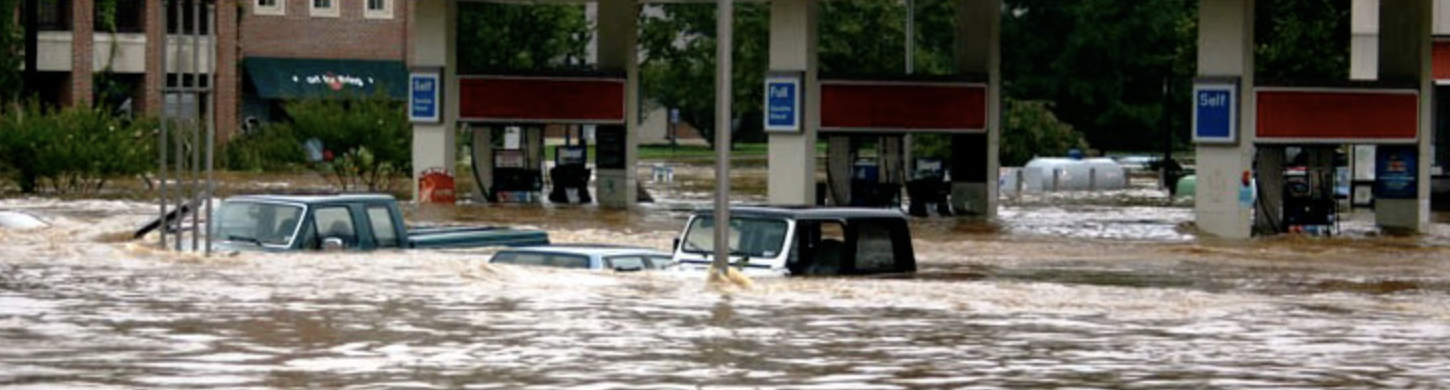
\includegraphics[width=1\linewidth]{Photo_2} \caption{Flooding in Asheville.}\label{fig:unnamed-chunk-2}
\end{figure}

\newpage

\hypertarget{dataset-information}{%
\subsection{\texorpdfstring{\textbf{Dataset
Information}}{Dataset Information}}\label{dataset-information}}

\hypertarget{discharge-data}{%
\subsubsection{\texorpdfstring{\textbf{Discharge
Data}}{Discharge Data}}\label{discharge-data}}

To understand the discharge in Asheville, North Carolina, we used data
from the United States Geographical Survey's (USGS) National Water
Information System (NWIS). We were able to pull this dataset into R
using the dataretrieval function which lets you simply put the specific
USGS code for the area we were interested in looking more closely at,
ours being the French Broad River. We chose stream gauge station
03451500 which is close to the city center of Asheville. There were
multiple parameters available for this site including discharge,
precipitation, pH, stream level, etc. By identifying the USGS code as
well as the specific codes for the parameters we wanted to look at
(i.e., discharge data) we were able to pull in corresponding data for
the last 60 years. Because discharge data is recorded daily, we had
records of every day from 1963 to 2021. The pulled dataset included the
agency (USGS), the site number, the date, and the amount of discharge in
cubic feet per second (Table 1).

Because we were able to pull in exactly which columns we wanted, there
was not much to wrangle for this specific dataset. We did however decide
that for all the parameters we were looking at that we would only
include the last forty years (1981-2021). In order to do this, we
filtered the dataset to only include those specific years. We also used
the lubridate package to change the date column to have a date class
format.

\hypertarget{precipitation-data}{%
\subsubsection{\texorpdfstring{\textbf{Precipitation
Data}}{Precipitation Data}}\label{precipitation-data}}

For precipitation data, we felt it was important to pull daily
precipitation data to better understand how extreme precipitation could
affect flash flooding of the French Broad River (Table 2). The dataset
we pulled is a csv file from the NOAA Global Historical Climatology
Network. When downloading the data, we were able to specify dates from
1981-2021 in order to obtain 40 years' worth of data so we could compare
earlier and later 20 year segments. This also helped us to match the
daily precipitation data to the daily discharge data we obtained from
the USGS National Water Information System.

In order to better understand what significant precipitation looked like
in Asheville, North Carolina, we read in another csv file from the NOAA
Precipitation Frequency Estimate Database. This table gave us
information about the 24-hour 1-year rainfall event, 2-year rainfall
event, and 5-year rainfall event (Table 5). With this knowledge, we were
able to explore whether extreme precipitation events (daily
precipitation over the 1-year, 2-year, and 5-year thresholds) had
increased over time and whether this impacted river discharge and flood
risk in the city.

\hypertarget{combined-data}{%
\subsubsection{\texorpdfstring{\textbf{Combined
Data}}{Combined Data}}\label{combined-data}}

For our linear model dataset, we combined both the discharge and the
precipitation datasets into one using the leftjoin function (Table 3).
Doing so, we had both the date, the amount of discharge in cubic feet
per second, and the precipitation in milliliters from the past 40 years.
For some reason, some of the precipitation entries were negative numbers
so we filtered to make sure the final dataset included only
precipitation values greater than 0 milliliters.

\newpage
\begin{table}
\centering
\begin{tabular}[t]{l|l|l|r}
\hline
\multicolumn{4}{c}{French Broad River USGS Discharge Data} \\
\cline{1-4}
Agency Code & Site Number & Date & Discharge\\
\hline
USGS & 03451500 & 1981-01-02 & 867\\
\hline
USGS & 03451500 & 1981-01-03 & 840\\
\hline
USGS & 03451500 & 1981-01-04 & 825\\
\hline
USGS & 03451500 & 1981-01-05 & 751\\
\hline
USGS & 03451500 & 1981-01-06 & 790\\
\hline
USGS & 03451500 & 1981-01-07 & 800\\
\hline
\multicolumn{4}{l}{\rule{0pt}{1em}\textit{Table 1: }}\\
\multicolumn{4}{l}{\rule{0pt}{1em}French Broad River USGS Discharge Data Table.}\\
\end{tabular}
\end{table}

\begin{table}
\centering
\begin{tabular}[t]{l|r|r|r}
\hline
\multicolumn{4}{c}{Asheville NOAA Precipitation Data} \\
\cline{1-4}
Date & Precip.mm & Month & Year\\
\hline
1981-01-01 & 0.3 & 1 & 1981\\
\hline
1981-01-02 & 0.0 & 1 & 1981\\
\hline
1981-01-03 & 0.0 & 1 & 1981\\
\hline
1981-01-04 & 0.0 & 1 & 1981\\
\hline
1981-01-05 & 0.0 & 1 & 1981\\
\hline
1981-01-06 & 0.0 & 1 & 1981\\
\hline
\multicolumn{4}{l}{\rule{0pt}{1em}\textit{Table 2: }}\\
\multicolumn{4}{l}{\rule{0pt}{1em}Asheville NOAA Precipitation Data Table.}\\
\end{tabular}
\end{table}

\begin{table}
\centering
\begin{tabular}[t]{l|r|r|r|r}
\hline
\multicolumn{5}{c}{Discharge and Precipitation Combined Data} \\
\cline{1-5}
Date & Precip.mm & Month & Year & Discharge\\
\hline
1981-01-01 & 0.3 & 1 & 1981 & NA\\
\hline
1981-01-07 & 0.3 & 1 & 1981 & 800\\
\hline
1981-01-15 & 0.5 & 1 & 1981 & 800\\
\hline
1981-01-20 & 5.6 & 1 & 1981 & 770\\
\hline
1981-01-21 & 0.3 & 1 & 1981 & 770\\
\hline
1981-01-27 & 2.3 & 1 & 1981 & 703\\
\hline
\multicolumn{5}{l}{\rule{0pt}{1em}\textit{Table 3: }}\\
\multicolumn{5}{l}{\rule{0pt}{1em}Discharge and Precipitation Combined Data.}\\
\end{tabular}
\end{table}

\begin{table}
\centering
\begin{tabular}[t]{l|l}
\hline
\multicolumn{2}{c}{Data Set Structure} \\
\cline{1-2}
Data & Data Types\\
\hline
Date & Date\\
\hline
Percip mm & Numeric\\
\hline
Month & Numeric\\
\hline
Year & Numeric\\
\hline
Discharge & Numeric\\
\hline
\multicolumn{2}{l}{\rule{0pt}{1em}\textit{Table 4: }}\\
\multicolumn{2}{l}{\rule{0pt}{1em}Data types of combined discharge and precipitation data.}\\
\end{tabular}
\end{table}

\newpage

\hypertarget{exploratory-analysis}{%
\subsection{\texorpdfstring{\textbf{Exploratory
Analysis}}{Exploratory Analysis}}\label{exploratory-analysis}}

\hypertarget{discharge-exploration}{%
\subsubsection{\texorpdfstring{\textbf{Discharge
Exploration}}{Discharge Exploration}}\label{discharge-exploration}}

In order to better understand the flood risk in Asheville, North
Carolina, we were interested in understanding the daily discharge data
throughout time (Figure 2) as well as the overall relationship between
discharge and precipitation. To measure this we wanted to run a time
series of the discharge data (Figure 4) as well as a seasonal
decomposition to understand both the seasonality of the data and the
trend throughout time. We also wanted to understand what in fact was the
trend over time and how this information can inform the flood risk for
Asheville.

As for the relationship between discharge and precipitation, we felt the
best way to see this was through a general linear model (Figure 9). By
looking at the dependence that discharge may have over precipitation, we
were confident that this too would help us to answer our original
research question of how these two parameters and the relationship
between them have impacted the flood risk over time.

\begin{figure}
\centering
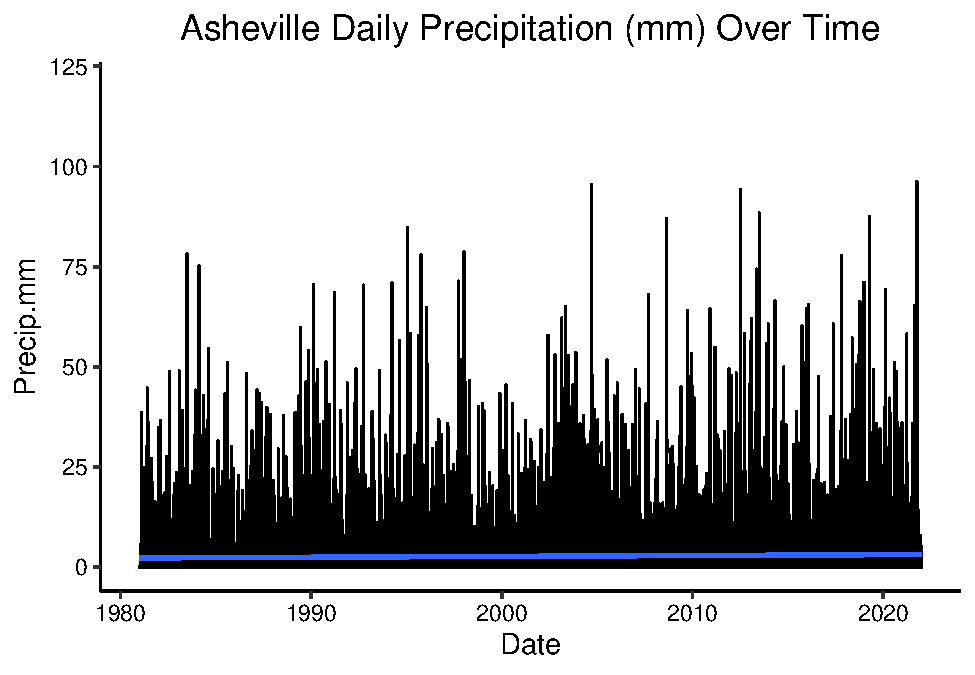
\includegraphics{SD_AD_NVT_EDAfinal_files/figure-latex/unnamed-chunk-7-1.pdf}
\caption{French Broad Discharge over time.}
\end{figure}

\hypertarget{precipitation-exploration}{%
\subsubsection{\texorpdfstring{\textbf{Precipitation
Exploration}}{Precipitation Exploration}}\label{precipitation-exploration}}

One of the first things we did with precipitation data was plot it over
time (Figure 3) to see if we could visually see an increase in
precipitation over time. This plot did not give us much valuable
information, so we decided to create filtered datasets to better see the
intense precipitation events above the 1-year, 2-year, and 5-year
thresholds (Table 5).

\begin{figure}
\centering
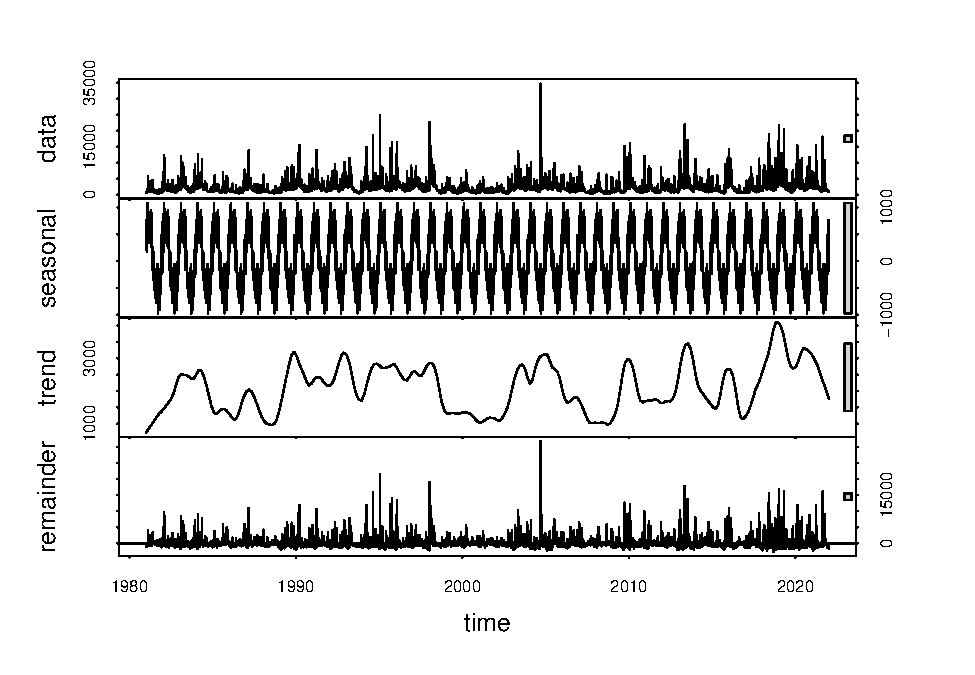
\includegraphics{SD_AD_NVT_EDAfinal_files/figure-latex/unnamed-chunk-8-1.pdf}
\caption{Asheville precipitation over time.}
\end{figure}

\newpage

\hypertarget{analysis}{%
\subsection{\texorpdfstring{\textbf{Analysis}}{Analysis}}\label{analysis}}

Through our analysis we became more familiar with the data and the
relationship between precipitation and discharge in Asheville.

The following analysis can be divided into three parts:

\begin{enumerate}
\def\labelenumi{\arabic{enumi}.}
\item
  How has discharge changed over time?
\item
  How has precipitation changed over time?
\item
  What is the relationship of discharge to precipitaion?
\end{enumerate}

\hypertarget{discharge-analysis}{%
\subsubsection{\texorpdfstring{\textbf{Discharge
Analysis}}{Discharge Analysis}}\label{discharge-analysis}}

To first look at the trends of discharge data over time, we ran a simple
timeseries that began on January 1, 1981, and ran through December 31,
2021, with a frequency of 365 days (Figure 4). Because this data had a
seasonal component, we examined the decomposition of this timeseries
data to get a better visual of the trend and seasonality throughout time
(Figure 6).

\begin{figure}
\centering
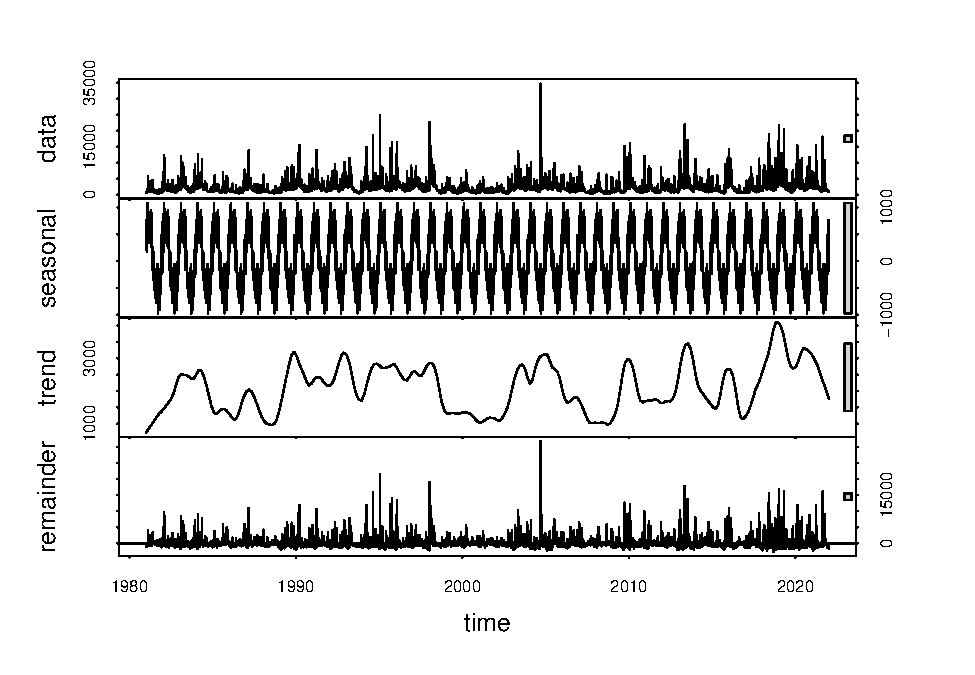
\includegraphics{SD_AD_NVT_EDAfinal_files/figure-latex/unnamed-chunk-9-1.pdf}
\caption{French Broad River discharge, time series decompostion.}
\end{figure}

After this, we created an ``Observed'' column in the dataframe to show
the discharge with the corresponding date so we could visualize both the
trend and the seasonality throughout time (Figure 5).

\begin{figure}
\centering
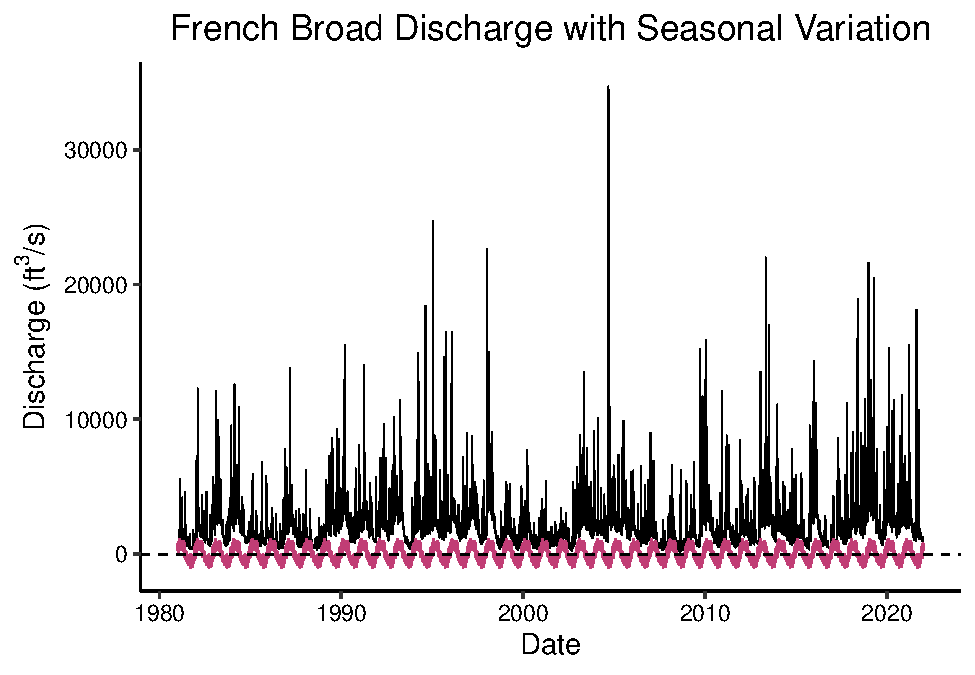
\includegraphics{SD_AD_NVT_EDAfinal_files/figure-latex/unnamed-chunk-10-1.pdf}
\caption{French Broad River Discharge, trend over time with trend line.}
\end{figure}

\begin{figure}
\centering
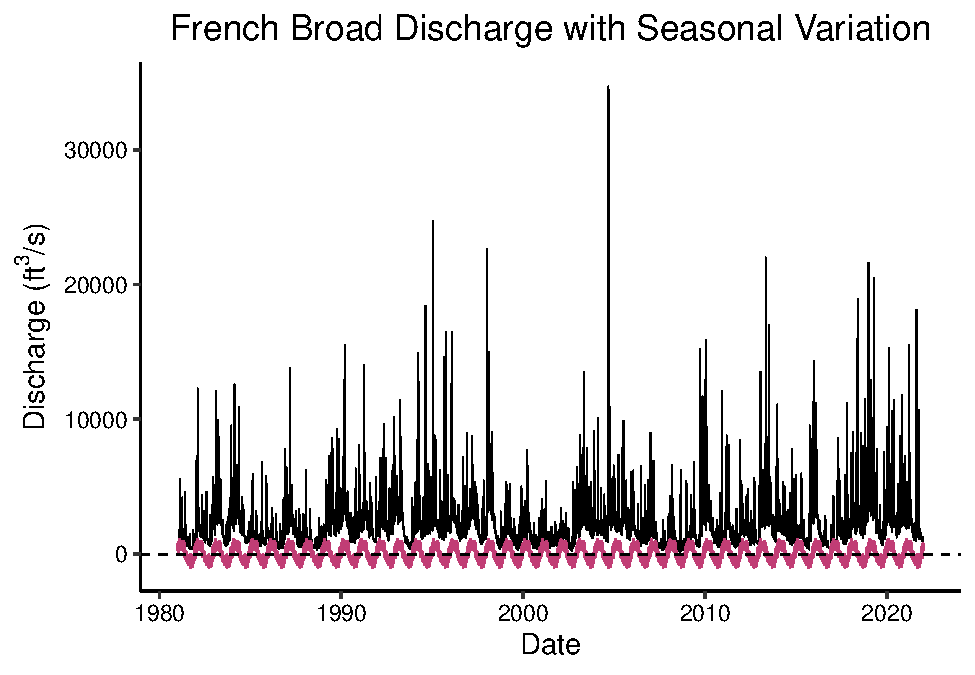
\includegraphics{SD_AD_NVT_EDAfinal_files/figure-latex/unnamed-chunk-11-1.pdf}
\caption{French Broad River Discharge, trend over time with seasonal
variation line.}
\end{figure}

Lastly, we used the Seasonal Mann-Kendall test to know whether the trend
over time was positive or negative. Our results of this test showed that
we could reject the null hypothesis that there is no trend in the
seasonal data and that there is a positive trend over time in the
discharge data (pvalue \textgreater{} 0.05, tau = 0.0622). The final
plot of the trend can be seen below.

\begin{figure}
\centering
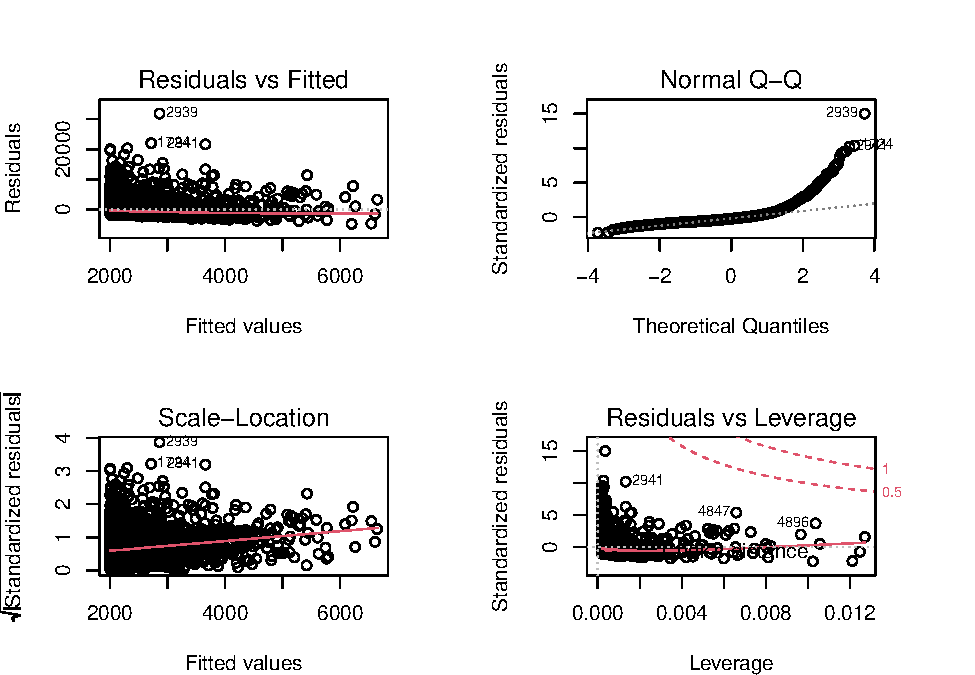
\includegraphics{SD_AD_NVT_EDAfinal_files/figure-latex/unnamed-chunk-12-1.pdf}
\caption{French Broad River Discharge, trend over time with line of best
fit.}
\end{figure}

\newpage

\hypertarget{precipitation-analysis}{%
\subsubsection{\texorpdfstring{\textbf{Precipitation
Analysis}}{Precipitation Analysis}}\label{precipitation-analysis}}

Filtering the data for the 1-year 24-hour precipitation events revealed
that more precipitation events over the 1-year 55mm threshold occurred
in the decades following 2000 than the decades preceding 2000.

This trend became more obvious as we increased the threshold of 24-hour
rainfall events to the 2-year 66mm level. The scatterplot and frequency
histogram revealed that the more intense rainfall events above the
2-year recurrence interval threshold were increasing in frequency.

Finally, we looked at the 5-year recurrence interval 24-hour rainfall
event and saw that of the 7 extreme precipitation events over the 5-year
82mm threshold, 6 occurred after 2000 and only one occurred before 2000.
Notably, the most extreme 24-hour precipitation event of the last 40
years occurred only last year in the fall of 2021.

Examining the precipitation data at the 1-year, 2-year, and 5-year
24-hour recurrence interval thresholds helped us to see that while there
wasn't a significant increase in overall precipitation over the last 40
years, more extreme rainfall events are occurring more frequently in the
last 20 years than in the previous two decades before 2000 (Figure 7).

\begin{table}
\centering
\begin{tabular}[t]{l|r|r|r|r|r|r|r|r|r|r}
\hline
\multicolumn{11}{c}{Significant Rainfall in Asheville, NC} \\
\cline{1-11}
Duration & 1 year & 2 year & 5 year & 10 year & 25 year & 50 year & 100 year & 200 year & 500 year & 1000 year\\
\hline
5-min: & 8 & 10 & 12 & 14 & 16 & 17 & 19 & 20 & 22 & 24\\
\hline
10-min: & 14 & 16 & 19 & 22 & 25 & 28 & 30 & 32 & 35 & 38\\
\hline
15-min: & 17 & 20 & 25 & 28 & 32 & 35 & 38 & 41 & 44 & 47\\
\hline
30-min: & 23 & 28 & 35 & 40 & 47 & 52 & 58 & 63 & 71 & 77\\
\hline
60-min: & 29 & 35 & 45 & 52 & 63 & 71 & 80 & 89 & 102 & 112\\
\hline
2-hr: & 33 & 40 & 51 & 59 & 71 & 81 & 91 & 102 & 117 & 129\\
\hline
3-hr: & 35 & 41 & 52 & 61 & 74 & 85 & 96 & 108 & 125 & 139\\
\hline
6-hr: & 41 & 48 & 60 & 70 & 84 & 96 & 109 & 123 & 143 & 159\\
\hline
12-hr: & 50 & 59 & 73 & 84 & 99 & 111 & 124 & 136 & 153 & 166\\
\hline
24-hr: & 55 & 66 & 82 & 95 & 112 & 125 & 139 & 153 & 171 & 184\\
\hline
2-day: & 66 & 79 & 97 & 111 & 130 & 145 & 160 & 175 & 194 & 209\\
\hline
3-day: & 70 & 84 & 102 & 116 & 136 & 151 & 165 & 180 & 199 & 213\\
\hline
4-day: & 74 & 89 & 107 & 122 & 141 & 156 & 171 & 185 & 204 & 217\\
\hline
7-day: & 87 & 104 & 125 & 141 & 163 & 180 & 196 & 213 & 234 & 249\\
\hline
10-day: & 100 & 118 & 141 & 158 & 181 & 199 & 216 & 234 & 255 & 271\\
\hline
20-day: & 138 & 162 & 189 & 210 & 237 & 258 & 278 & 297 & 321 & 338\\
\hline
30-day: & 172 & 201 & 230 & 252 & 279 & 299 & 318 & 335 & 357 & 371\\
\hline
45-day: & 218 & 255 & 286 & 310 & 338 & 358 & 376 & 393 & 412 & 424\\
\hline
60-day: & 262 & 305 & 341 & 366 & 398 & 420 & 439 & 457 & 477 & 490\\
\hline
\multicolumn{11}{l}{\rule{0pt}{1em}\textit{Table 5: }}\\
\multicolumn{11}{l}{\rule{0pt}{1em}Significant rainfall events in Asheville, NC.}\\
\end{tabular}
\end{table}

\begin{figure}
\centering
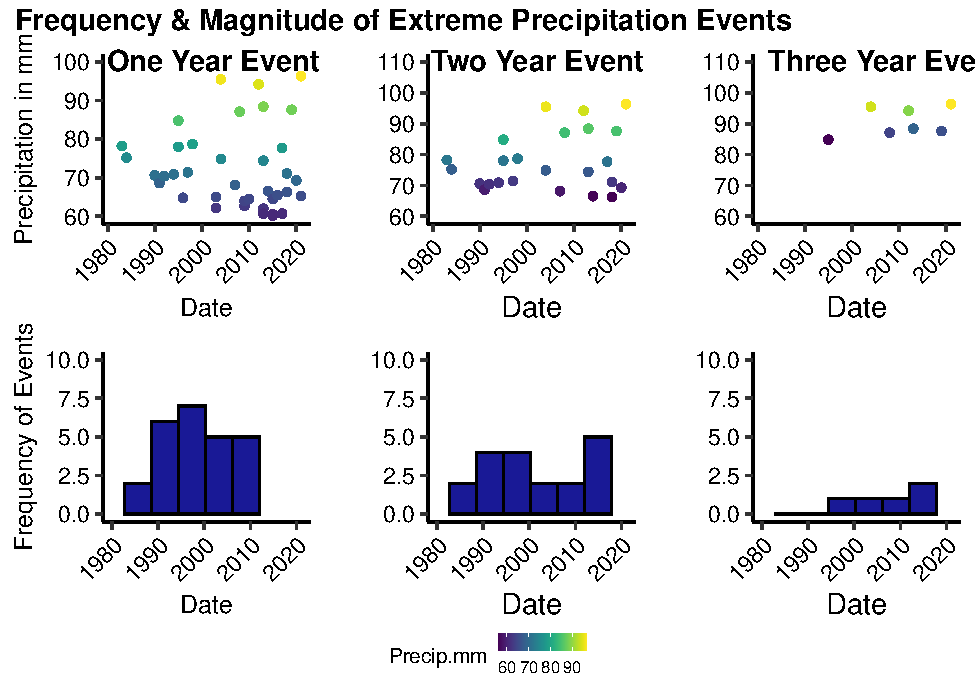
\includegraphics{SD_AD_NVT_EDAfinal_files/figure-latex/unnamed-chunk-14-1.pdf}
\caption{Frequency and magnitude of precipitation events over time.}
\end{figure}

\newpage

\hypertarget{discharge-and-precitpitaion-relationship}{%
\subsubsection{\texorpdfstring{\textbf{Discharge and Precitpitaion
Relationship}}{Discharge and Precitpitaion Relationship}}\label{discharge-and-precitpitaion-relationship}}

In our next analysis, we looked more at the relationship between
discharge and the precipitation data. As mentioned previously, we used a
general linear model to look more closely at this relationship. Our
results of this linear model regression show that there was in fact a
significant relationship between the two variables, and we were
confidently able to reject the null hypothesis that there was no
relationship between discharge and precipitation. It can be seen below
in the QQ-Plot that this data is not really normally distributed and
that it would be advantageous to potentially log-transform the data to
view the relationship better (Figure 8).

\begin{figure}

{\centering 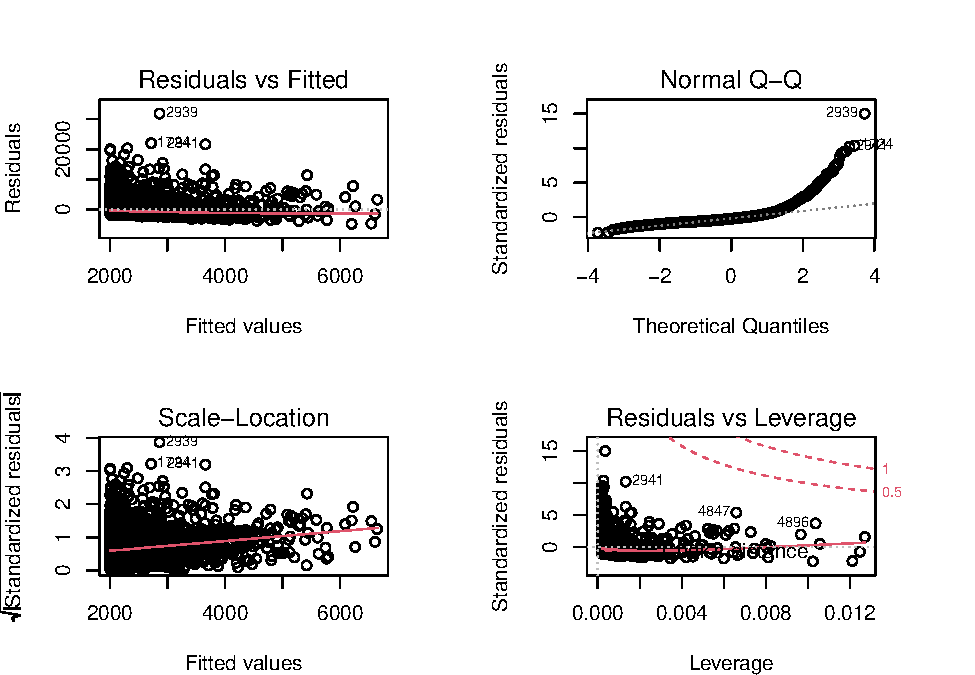
\includegraphics{SD_AD_NVT_EDAfinal_files/figure-latex/unnamed-chunk-15-1} 

}

\caption{French Broad River discharge and Asheville precipitation, linear model results.}\label{fig:unnamed-chunk-15}
\end{figure}

Looking closer at the linear model results, we were able to determine
that this was a positive relationship and that for every one unit of
precipitation, discharge increased by 48.3 cubic feet per second
(p-value \textless{} 0.05, F-statistic = 324.3 on 1 and 525 degrees of
freedom, R\^{}2 = 0.05805). Our R-squared value however only explained
around 6\% of the variability and this could be due to the fact that
discharge and precipitation isn't usually modelled linearly which could
account for the lower R\^{}2 and could be something to investigate
further. A detailed visualization of the relationship can be seen in the
plot below (Figure 9).

\begin{figure}
\centering
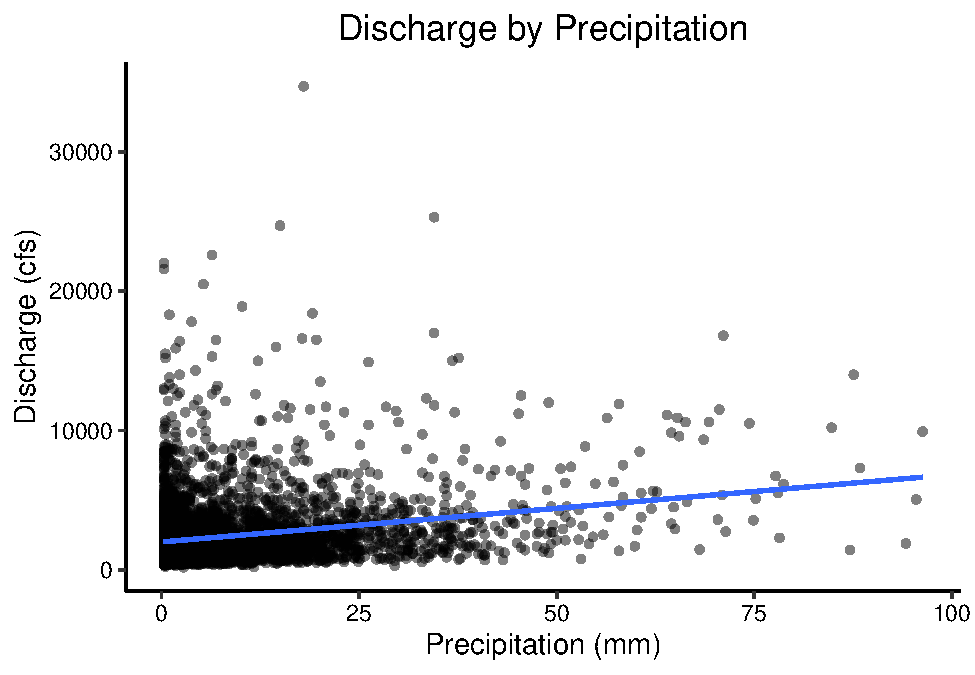
\includegraphics{SD_AD_NVT_EDAfinal_files/figure-latex/unnamed-chunk-16-1.pdf}
\caption{French Broad River discharge by Asheville precipitation, linear
relationship.}
\end{figure}

Both of these analyses can be helpful to inform our original research
question of how these variables and the relationship between them have
changed over time and will be discussed at greater length in our summary
and conclusion sections.

\newpage

\hypertarget{summary-and-conclusions}{%
\subsection{\texorpdfstring{\textbf{Summary and
Conclusions}}{Summary and Conclusions}}\label{summary-and-conclusions}}

Through our analysis we observed how precipitation and river discharge
are changing in Asheville over time. Even though there may be an
increase of flooding events that, does not always correlate to an
increases in precipitation and discharge as large events could be
balanced by period of lower than normal rainfall. Our analysis did allow
us to answer our research questions and gain a better understand of
hydrologic events in Asheville in the past 40 years.

Through our analysis of discharge in the French Broad river we were able
to answer our first research question of what trends exist in discharge
data over time. We found that although small, there is indeed an
increase in overall discharge moving through the French Broad river in
the past 40 years. After decomposing our time series analysis we found
that the trend of the overall data was not clearly increasing. We did
however find that there was a slight visual correspondence between the
seasonal data and the overall shape of the time series plot. This
finding was confirmed with the results of the Seasonal Man Kendall test.
Our results of this test showed that we could reject the null hypothesis
that there is no trend in the seasonal data and that there is a positive
trend over time in the discharge data, answering our second research
question.

Analysis of the precipitation data in Asheville resulted in a result of
a positive increase in the frequency of extreme precipitation events
over time, answering research questions number three (Figure 3).
Additionally, we looked at the frequency of the 24-hour rainfall event
at the one-year, two-year, and five-year recurrence interval. We found
that over the past 40 years, more intense precipitation events over the
1-year, 2-year, and 5-year thresholds have been increased in frequency.
At the most extreme end of our analysis, the five-year rainfall event,
we found that daily rainfall has exceeded this threshold almost
exclusively in the past 20 years. This analysis allowed us to answer our
fourth and firth research questions. We can conclude that intense
rainfall events are increasing over time in Asheville (Figure 7).

An analysis of the relationship between precipitation and river
discharge gave us a significant result answering our sixth research
question. As one would suspect, precipitation has a positive effect on
river discharge. This result provides further evidence that the
increases measured in precipitation event magnitude and frequency will
also have an increase in magnitude and frequency of high discharge in
the river (Figure 9).

The changing climate puts to the test the systems that have been built
around data from the past. Acknowledging these increases in hyrodologic
activity, which lead to an increase in flood risk, requires
municipalities to assess their current storm water system and flood
plain boundaries. Awareness of the changing conditions is necessary for
communities to be able to adapt and build resilience to climate risks in
their areas.

\begin{figure}

{\centering 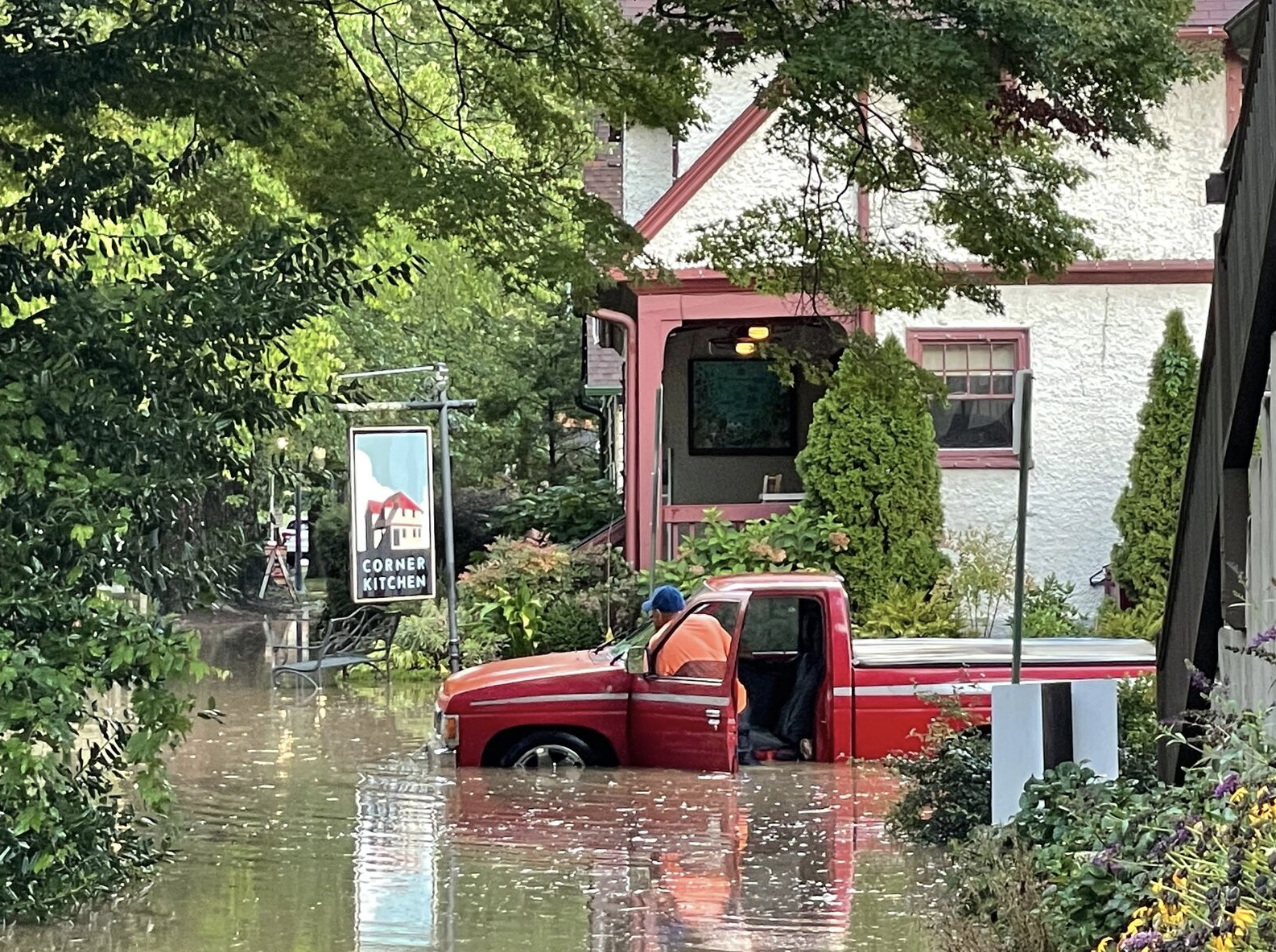
\includegraphics[width=0.75\linewidth]{Photo_1} 

}

\caption{Flooding in Asheville.}\label{fig:unnamed-chunk-17}
\end{figure}

\newpage

\hypertarget{references}{%
\subsection{\texorpdfstring{\textbf{References:}}{References:}}\label{references}}

Harris, S. (2021, August 20). Asheville and Buncombe flooding related
road, park closures, Help Line. The Asheville Citizen Times. Retrieved
April 16, 2022, from
\url{https://www.citizen-times.com/story/news/2021/08/20/asheville-buncombe-nc-area-flooding-road-park-closures-help-line/8211528002/}

FloodFactor (2022). Asheville, North Carolina. Flood Factor.
\url{https://floodfactor.com/city/asheville-northcarolina/3702140_fsid}

Figure 1: Photo credit:
\url{https://www.ashevillenc.gov/department/public-works/stormwater-services-utility/flood-information/}

Figure 2: Photo credit: Amy Westmoreland

\end{document}
